\documentclass[12pt,letterpaper,oneside]{book}
\title{AFIT-ENY-MS-19-M-XXX_LeSieur_new}
\usepackage{FrontMatter/afitThesis}
\usepackage{FrontMatter/sf298}
\usepackage{booktabs, multirow, tabularx} %tables
\usepackage{adjustbox} %rotates pictures in a document
\usepackage{subfig} %puts pictures side-by-side
\usepackage{float}
\usepackage{placeins}
\usepackage{gensymb}
\usepackage{nicefrac}
\usepackage{graphicx}
\usepackage{verbatim} %allows for multi-line comments: begin{comment}...end{comment}
\usepackage[capitalise,noabbrev]{cleveref}
\usepackage{setspace}
\usepackage[nocompress]{cite}
\usepackage{caption}
%Picture Borders
\setlength{\fboxsep}{0pt} 
\setlength{\fboxrule}{1pt}
%

\allowdisplaybreaks %Spacing with pictures, place after amsmath
%Create line through V symbol \volume
\makeatletter
\DeclareRobustCommand{\volume}{\text{\volumedash}V}
\newcommand{\volumedash}{%
  \makebox[0pt][l]{%
    \ooalign{\hfil\hphantom{$\m@th V$}\hfil\cr\kern0.08em\textbf{--}\hfil\cr}%
  }%
}
\makeatother

%Prevent paragraph indent directly after figure
\makeatletter
\renewcommand\float@endH{\@endfloatbox\vskip\intextsep
  \if@flstyle\setbox\@currbox\float@makebox\columnwidth\fi
  \box\@currbox\vskip\intextsep\relax\@doendpe}
\makeatother

 
% =========================== Input ==========================
\author{Alexander R. LeSieur}
\rank{Captain, USAF} 
\docdesignator{AFIT-ENY-MS-19-M-XXX}
\department{Department of Aeronautics and Astronautics}
\graduationdate{XX March 2019} %\today
\title{\MakeUppercase{Fragmentation Properties of Explosively Driven Additively Manufactured Metals}}
\previousdegrees{BSAE}
\acdegree{Master of Science in Aeronautical Engineering}
\committee{{Major , PhD\\Chair},
		   {Dr. , PhD\\Member},
           {Dr. , PhD\\Member}}
\address{2950 Hobson Way\\ Air Force Institute of Technology \\
Wright-Patterson AFB, OH 45433}
\distribution{DISTRIBUTION STATEMENT A\\[-10pt]
\MakeUppercase{Approved for Public Release; distribution unlimited.}
} 
\disclaimer{The views expressed in this document are those of the
author and do not reflect the official policy or position of the
United States Air Force, the United States Department of Defense or
the United States Government.  This material is declared a work of the
U.S. Government and is not subject to copyright protection in the
United States.}

 %Title Pg Inputs
%-----------------------------------------------------------------------
% Ch1 Acronyms

\newacronym{AM}{AM}{Additive Manufacturing}
\newacronym{CAD}{CAD}{Computer-aided Design}
\newacronym{DIC}{DIC}{Digital Image Correlation}
\newacronym{DoD}{DoD}{Department of Defense}
\newacronym{EBW}{EBW}{Exploding-Bridgewire Detonator}
\newacronym{PH}{PH}{Precipitation Hardening}
\newacronym{DMLS}{DMLS}{Direct Metal Laser Sintering}
\newacronym{SLM}{SLM}{Selective Laser Melting}
\newacronym{SNL}{SNL}{Sandia National Laboratories}
\newacronym{USAF}{USAF}{United States Air Force}
%-----------------------------------------------------------------------
% Ch2 Acronyms
\newacronym{fps}{fps}{frames per second}
\newacronym{EDM}{EDM}{Electrical Discharge Machining}
\newacronym{KE}{KE}{Kinetic Energy}
\newacronym{PBF}{PBF}{Powder Bed Fusion}
\newacronym{DPV}{DPV}{Photonic Doppler Velocimetry}
\newacronym{SLS}{SLS}{Selective Laser Sintering}
\newacronym{PETN}{PETN}{Pentaerythritol Tetranitrate}
%-----------------------------------------------------------------------
% Ch3 Acronyms




%-----------------------------------------------------------------------
% Ch4 Acronyms




%-----------------------------------------------------------------------
% Ch5 Acronyms
 


\begin{document}

%\frontmatter
 %    \flyleaf
    % \disclaimerpage
    % \titlepageAFIT
    % \committeepage
 %    \begin{abstract}

Fragmentation properties are a crucial component of military weaponeering, where the fundamental goal is to create the optimal weapons package for mission accomplishment, while minimizing collateral damage. Additive manufacturing presents an avenue towards tailoring a warhead's design to a specific target set, allowing weapons experts to develop efficient attack solutions, further reducing unintended consequences, while improving aircraft survivability. Understanding the fragmentation properties of additively manufactured materials under explosive loading is needed before they are utilized in weaponry applications. This research will examine the fracture behavior of metal casings produced by additive manufacturing and the resulting fragment velocity and mass distributions through experimental analysis.

\end{abstract} 
    % \begin{acknowledgements}
\begin{center}

....

\end{center}
\end{acknowledgements} 
    % \tableofcontents 
    % \listoffigures          
    % \listoftables    
    % \singlespacing
    % \printglossary[type=\acronymtype,title=List of Acronyms,toctitle=List of Acronyms] 
    % \addtocontents{toc}{\vspace{0.4\normalbaselineskip}}
    % \renewcommand{\nomname}{List of Symbols}\printnomenclature
    % \doublespacing

\mainmatter	
	\chapter{Introduction} \label{chap:1}

%-----------------------------------------------------------------------
\section{Background}
%-----------------------------------------------------------------------

Since the end of the Second World War, the \gls{USAF} has emphasized reducing collateral damage and increasing aircraft survivability in combat operations \cite{SurvivabilityArticle,CollateralDamageNPS}. These two efforts are not always complementary, as the weapons package needed for minimal risk of civilian casualties may demand the use of additional military personnel and airframes. This creates a great burden for military commanders, who must delicately balance \gls{DoD} policies and potential political ramifications with subjecting humans and expensive assets to hostile environments. Therefore, armament selection is of paramount importance when planning attack missions. 

Current military strategy constrains weapons experts to employing munitions with predetermined explosives capacities. After considering parameters such as warhead size and body construction, experts can estimate the number of munitions required to impose a desired level of damage against the target of interest, formulating a ``weapons package." While this process is usually sufficient when engaging large-scale isolated targets, issues arise when a strike is required in a dynamic environment featuring civilian populations and/or nonmilitary structures and assets. In these situations, the issues of fragmentation patterns and blast effects manifest as potential sources of unintended consequences. Understanding and controlling these factors play a significant role in modern military weaponeering and in particularly warhead design. 

Warhead design encompasses all aspects of developing and building the explosive unit contained within a munition. Although weapon detonation events involve complex interactions between the explosive charge and the warhead casing, fragmenting munitions generally exhibit a predictable detonation sequence. As the explosives inside a munition's warhead are detonated, the energy released from the rapid exothermic (release of heat) reaction generates pressure on the weapon’s casing, causing it to expand and experience material deformation. Once the stresses imparted on the casing exceed the material’s strength, the weapon’s internal structure fails and fractures. This leads to the formation of fragments, which are accelerated and propelled to the target by explosive gases created during the detonation \cite{Cooper1996}. Material properties are a driving factor behind the casing’s fracture behavior and fragment velocity, which ultimately determine the lethality and effectiveness of a given munition’s design. Traditional weapon casing production utilizes conventional metal fabrication methods (ex. casting, forging, etc.); however, \gls{AM} introduces...  

%A potential 

\gls{AM} refers to any production technique where a component is constructed in a vertical build direction using a sequential layering scheme \cite{OverviewofAM_OHara}. In most situations, the user first virtually models the component in a \gls{CAD} software package, which is then exported to the \gls{AM} machine, providing a manufacturing blueprint. While there are many different methods of \gls{AM}, \gls{DMLS} was selected to build the test specimens in this research, due to its well-established history amongst \gls{AM} methods and its ability to print metal components. In \gls{DMLS}, components are constructed using a laser and fine powder. First, the machine ``slices" the supplied \gls{CAD} model into thin cross sectional layers, creating a specific scan strategy (how the laser moves over each individual layer). Then, a thin layer of metal powder is deposited on a build plate, before the machine's laser heats and sinters the powder along a build path determined by the cross sectional layers. As the sintered powder cools, a solid structure forms, and the process is repeated in a series of sequential layers until the entire component is fully constructed.

Since \gls{AM}-produced parts are built on top of a freestanding substrate (plate which serves as surface for the machine to deposit material) in lieu of a predefined mold, the builder can make modifications or construct an entirely new component simply by exporting an updated \gls{CAD} file to the machine. This significantly simplifies both the manufacturing process and the ability to alter a component's design, making \gls{AM} inherently customizable in nature \cite{Furumoto}.
 
%-------------------------------------------------------------------
\section{Motivation}
%-----------------------------------------------------------------------
Warhead and weapons design are foundational in the study of military weaponeering. Explosive capacity, blast effects, and fragmentation pattern (how the weapon breaks apart after it is detonated) heavily contribute to a weapon's and overall effectiveness and employability in combat operations. While the \gls{DoD} has a wide of array of munitions of varying sizes and explosive capabilities in its current arsenal, there is currently no widespread solution for designing munitions around a specific target. \gls{AM} presents a potential pathway to maximum weapon effectiveness by allowing munitions experts to custom-build munitions for a given mission. By optimizing weapons and their associated effects around the mission itself, targeteers and weapons experts could formulate attack strategies which require the least amount of assets and personnel as possible, while minimizing collateral damage.  

Currently, there is very little documented research regarding incorporating \gls{AM}-printed metals into applications involving explosive environments. Distinct fabrication techniques commonly found in \gls{AM} create unique internal features not normally found in conventional production methods. For instance, at least a small amount of defects and micropores are always present in additively manufactured materials due to interactions between the laser, powder, and previously deposited layers \cite{ChoiSLMDensity}. Before integrating \gls{AM} into weaponry design, further research needs to investigate the behavior of additively manufactured metals under an explosive loading to determine if \gls{AM} is a suitable method for warhead construction.


%-----------------------------------------------------------------------
\section{Problem Statement}
\label{ProblemStatement}
%-----------------------------------------------------------------------

In modern military combat operations, the extensive use of explosive weaponry can cause collateral damage, especially when the target is within close proximity to civilian populations. To mitigate unintended consequences, military targeteers must formulate ``weapons packages" to achieve mission success with the minimum amount of firepower necessary. Unfortunately, they are currently limited to utilizing only ready-made weapons with pre-determined capabilities, meaning the munitions are not specifically designed for the target of interest. Coupled with the need to balance objectives with rules of engagements, commanders may need to add additional sorties and aircraft to ensure mission completion, increasing exposure to enemy fire. By incorporating \gls{AM} into warhead design, weapons experts could custom-build munitions for a specific target set, increasing attack efficiency and aircraft survivability while further reducing unintended consequences \cite{SurvivabilityArticle}. 


%-----------------------------------------------------------------------
\section{Scope \& Objectives}
%-----------------------------------------------------------------------

The focus of this research is to investigate and analyze the deformation and fragmentation behavior of \gls{AM}-printed metal cylindrical casings subjected to an explosive loading. The primary properties studied in this experiment are material fragmentation velocity and resulting fragment mass distribution; however, strain rates calculated during the detonations will also yield information regarding the material's ductility and resistance to fracture. After testing is complete and material properties are calculated, follow-on analysis will compare collected data with established fragmentation theories and equations, providing a better understanding of how additively manufactured metals perform in explosive environments. The scope of this research is obtained by adhering to the following objectives:

\begin{enumerate}
\item Detonate \gls{AM}-printed cylindrical casings and record test events using high-speed imaging
\item Analyze casing reactions to explosive loading using diagnostic tools and to determine material properties 
\item Compare the fragmentation behavior of the additively manufactured samples to conventionally produced metals using traditional fragmentation theories and equations
\end{enumerate}

%-----------------------------------------------------------------------
\section{Methodology}
%-----------------------------------------------------------------------

\gls{CAD} models of the desired test samples were provided to Oregon-based \gls{AM} company I3DMFG for machining using 15-5PH Stainless Steel powder. In total, 90 samples were produced and ultimately tested at \gls{SNL} in Albuquerque, New Mexico. Before they were detonated, the test specimens were loaded with the explosive \gls{PETN}, coupled with \glspl{EBW}. Finally, samples were detonated inside specialized indoor blast chambers, where the casing expansion and fragmentation events were captured using multiple high-speed cameras \cite{TeledyneRP-80}. Following each test, the resulting fragments were collected and individually weighed for follow-on mass distribution analysis. This process was repeated until all samples were detonated.
  
Following test completion, the collected experimental data underwent \gls{DIC} analysis. \gls{DIC} is a non-contact optical tracking method which captures the deformation and fracture behavior of materials in motion \cite{DICimageObservations}. This is accomplished by ``following" pixel movements between multiple images. Due to its ability to quantify material behavior in dynamic environments (materials in motion), \gls{DIC} is extremely useful for calculating material strain and fragment velocity \cite{ReuDICapplication}. For this research, \gls{DIC} was performed on images obtained by the high-speed cameras to track casing expansion and movement of fragments resulting from the explosive detonation.  

Results obtained from \gls{DIC} analysis were compared to fragmentation models of conventional metal casings developed in previous research to determine if additively manufactured metals are suitable for use in explosives applications. The primary fragmentation equations used for comparison purposes were the Gurney cylindrical casing equation and Mott fragmentation model (further detailed in Chapter II), which are heavily utilized in weaponeering and explosives research to predict fragment velocity and size/mass distribution, respectively.

%-----------------------------------------------------------------------
\section{Thesis Outline}
%-----------------------------------------------------------------------

This chapter provided a brief overview of the research presented in this thesis and why it is relevant to \gls{USAF} and \gls{DoD} interests. The following chapter presents a detailed review of the background and theory applicable to this research. Chapter III covers the methodology behind the research's data collection techniques, while the actual results are provided in Chapter IV. Finally, analysis and a summary of the results is covered in Chapter V, along with a discussion of recommended future research efforts.   
	\chapter{Background \& Theory} \label{chap:2}
 
In modern \gls{DoD} air combat operations, collateral damage and aircraft survivability estimates significantly influence the tactics and procedures utilized during any given attack mission. Consequently, military commanders and weaponeering experts must prepare armament packages which present the smallest amount of risk to civilian populations and structures, while exposing the least amount of military personnel and assets to hostile environments. Currently, the \gls{DoD} and \gls{USAF} are unable to custom build weapons for specific targets in a timely and efficient manner, meaning most missions rely on ready-made munitions not designed for unique circumstances. 

Modern military aircraft armament is produced using traditional metal processing methods, such as forging or casting. These techniques feature pre-determined molds or shaping instructions which require machine and assembly downtime to modify, making them unsuited for frequently changing requirements. By contrast, \gls{AM} enables manufacturers to customize and adjust part dimensions and features to customer requirements. Applying this to military weaponeering, \gls{AM} provides a potential solution to materializing a customized bomb-building capability. Since \gls{AM} and warhead design are largely studied independent of one another, there is little documentation on how \gls{AM}-printed metals respond to explosive detonations. This research seeks to investigate the performance of additively manufactured metal casings undergoing explosive loading. Classic fragmentation theories developed by R.W. Gurney and N.F. Mott provide a foundation to characterize experimental results and compare additively manufactured casing performance with traditional metal production methods. High speed photography and subsequent \gls{DIC} analysis visually capture and quantify the metal's mechanical properties, bringing awareness to \gls{AM}'s suitability in weaponeering applications.



%-----------------------------------------------------------------------
\section{Additive Manufacturing} \label{sec:2_AdditiveManufacturing}
%-----------------------------------------------------------------------

\gls{AM} is an umbrella term used to describe fabrication techniques which produce components through a progressive layering process. Colloquially referred to as ``3D printing," \gls{AM} is becoming increasingly common in a wide array of industries as it becomes a more economical and reliable production method. Although there are several different types of \gls{AM} processes, each having its own construction method and resulting material characteristics, \gls{PBF} was selected for this research.

% Although there are several different types of \gls{AM} processes, each having its own construction method and resulting material characteristics, \gls{SLM} was selected for this research.

%%%%%%%%%%%%%%%%%%%%%%%%%%%%%%%%%%%%
\subsection{\glsentryfull{PBF}} \label{sec:2_PBF}
%%%%%%%%%%%%%%%%%%%%%%%%%%%%%%%%%%%%

% %%%%%%%%%%%%%%%%%%%%%%%%%%%%%%%%%%%%
% \subsection{Selective Laser Melting} \label{sec:2_SLM}
% %%%%%%%%%%%%%%%%%%%%%%%%%%%%%%%%%%%%

\gls{PBF} machines, illustrated in \Cref{fig:2_PBF_Setup}, fabricate parts in a successive layering system using deposited powder and a directional laser heat source. First, a desired part's \gls{CAD} model is uploaded into the \gls{PBF} machine, which divides the model into cross-sectional layers, converting it into a series of individual layer blueprints. For each layer, the machine then maps the optimal laser path needed to achieve a desired level of quality, creating the overall scan strategy.

% \gls{SLM} machines, illustrated in \Cref{fig:2_SLM_Setup}, fabricate parts in a successive layering system using deposited powder and a directional laser heat source. First, a desired part's \gls{CAD} model is uploaded into the \gls{SLM} machine, which divides the model into cross-sectional layers, converting it into a series of individual layer blueprints. For each layer, the machine then maps the optimal laser path needed to achieve a desired level of quality, creating the overall scan strategy.

% PBF Machine Illustration
\begin{figure}[H]
	\centering
 \fbox{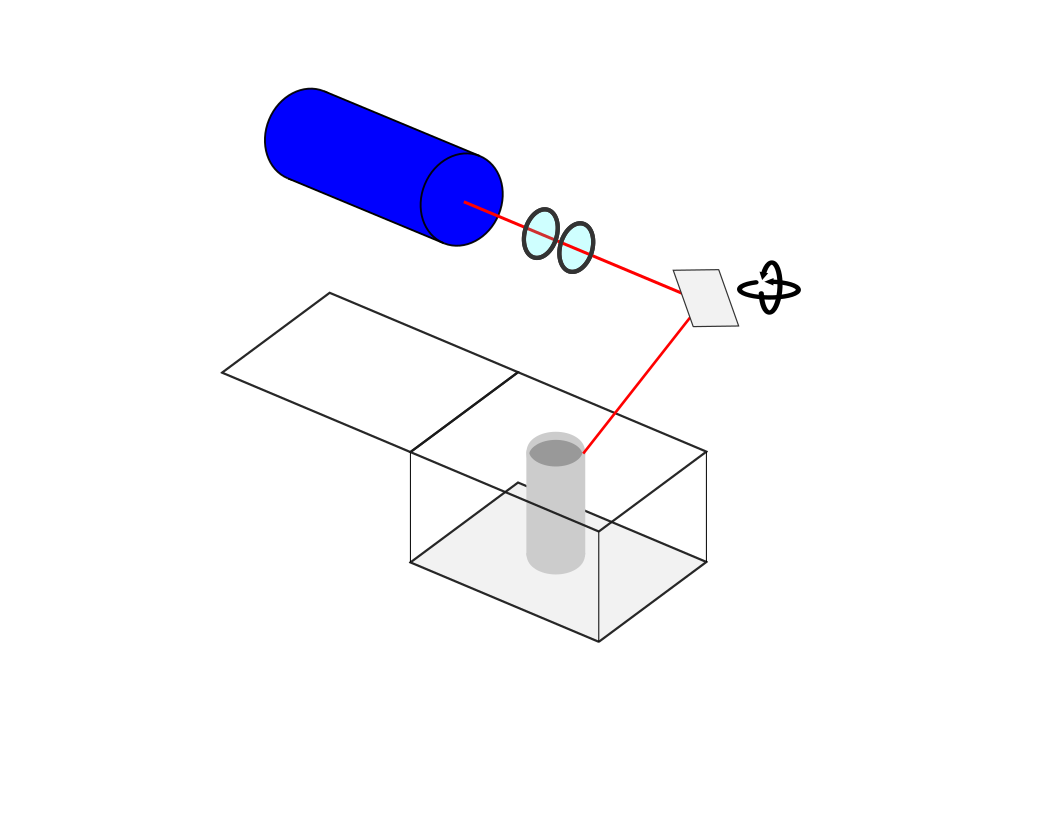
\includegraphics[width=0.7\linewidth]{Ch2/Figures/PBF_Setup.png}}
    \caption{Illustration of an \gls{PBF} machine, based on an illustration presented in \textit{The metallurgy and processing science of metal additive manufacturing} \cite{OverviewofAM_OHara} 
    \textbf{rough draft note: I am still working on drawing this, so it is incomplete}}
	\label{fig:2_PBF_Setup}
\end{figure}
%

Once the \gls{PBF} machine generates a manufacturing solution, an emitted laser is guided along the build path using a lens configuration and scanning mirror. The laser's energy rapidly heats and melts the deposited powder, which forms a solid layer upon cooling. After the laser completes the layer's build path, the powder platform is raised while the build platforms lowers by the length of one layer thickness. Next, the recoater blade spreads a layer of powder metal across the build platform, depositing new material on top of the previously scanned layer. The laser then maneuvers along the ensuing layer's build path, and the process is repeated until the entire part is constructed \cite{OverviewofAM_OHara}.

One of the most common \gls{PBF} techniques is \gls{DMLS}, a laser-based \gls{AM} method attributed to metal \gls{PBF} systems built by the German company EOS GmbH. Although they are named after the sintering process (fusing materials at temperatures slightly below their melting temperature) originally used by first generation printers in the mid-1990's, modern \gls{DMLS} manufacturing completely melts the deposited powder (EOS, private communication), making it equivalent to \gls{SLM} \cite{EOS_DMLS_History}.  

The primary advantage of \gls{DMLS} over sintering-based \gls{PBF} techniques, such as \gls{SLS}, is its ability to achieve relative densities of approximately 100 \% \cite{EOS_StainlessSteel_M290}. Compared to \gls{DMLS}, \gls{SLS} uses lower powered lasers which do not fully melt the build material, resulting in lower density components with inferior strength properties \cite{SLS_not_fully_dense}. Since \gls{DMLS} is a metal-based \gls{AM} technique, commonly used powders include aluminum, nickel, stainless steel, and titanium-based alloys. ...For high temperature and stress applications, 15-5 \gls{PH} stainless steel...

%Paragraph on 15-5 powder
15-5 \gls{PH} stainless steel is a martensitic steel alloy originally designed by Aramco (now AK Steel) as an improved variation of 17-4 \gls{PH} stainless steel. Since it lacks the weaker ferrite crystal structure found in 17-4 \gls{PH} stainless steel, 15-5 \gls{PH} stainless steel exhibits favorable strength properties  \cite{AKSteel_Conventional_SS,Ferrite_weaker}.
Following construction completion, 15-5 \gls{PH} stainless steel components are typically heat treated at a temperature between 900 and 1150 \degree F, significantly strengthening the components at a slight expense to material ductility \cite{AKSteel_Conventional_SS,EOS_StainlessSteel_M290}.  

%Unlike  sintered , \gls{DMLS} parts feature near full density

%%%%%%%%%%%%%%%%%%%%%%%%%%%%%%%%%%%%
\subsection{Powder Bed Fusion Drawbacks} \label{sec:2_PBF_drawbacks}
%%%%%%%%%%%%%%%%%%%%%%%%%%%%%%%%%%%%
While \gls{PBF} gives the manufacturer significant control over design parameters, the presence of a continuously-moving heat source (laser) introduces several sources of variability not found in conventional machining methods. For instance, prior research has shown variations in laser scan speed alone can have profound effects on the final part's porosity levels \cite{ChoiSLMDensity}. Additionally, entrapped gases, as well as size and shape variations in the powder feedstock further promote micropore formation \cite{Aboulkhair2014_microscopic_pores}. Other possible issues in \gls{PBF} include delamination (layer separation), cracking, and residual stress buildup. The presence and frequency of effects is controlled by laser power, powder feedstock quality, scan strategy, and various \gls{PBF} machine parameters \cite{OverviewofAM_OHara}. Together, these imperfections weaken the printed component's overall strength, which translates to impacting the casing's ability to withstand explosive loadings in this research.

Roberts et al. tensile tested \gls{DMLS} and wrought 15-5 \gls{PH} stainless steel cylindrical rods at elevated temperatures (593 \degree C) and noted while \gls{DMLS}-printed samples exhibited superior yield strength (...MPa vs ...Mpa) and ultimate tensile strength (...MPa vs ...Mpa) values, wrought samples displayed greater elongation percentages at fracture (..\% vs ..\%), suggesting \gls{DMLS} processing reduces material ductility \cite{Roberts_Traditional_AM_15_5_testing}. 

% PBF Machine Illustration
\begin{figure}[H]
	\centering
 \fbox{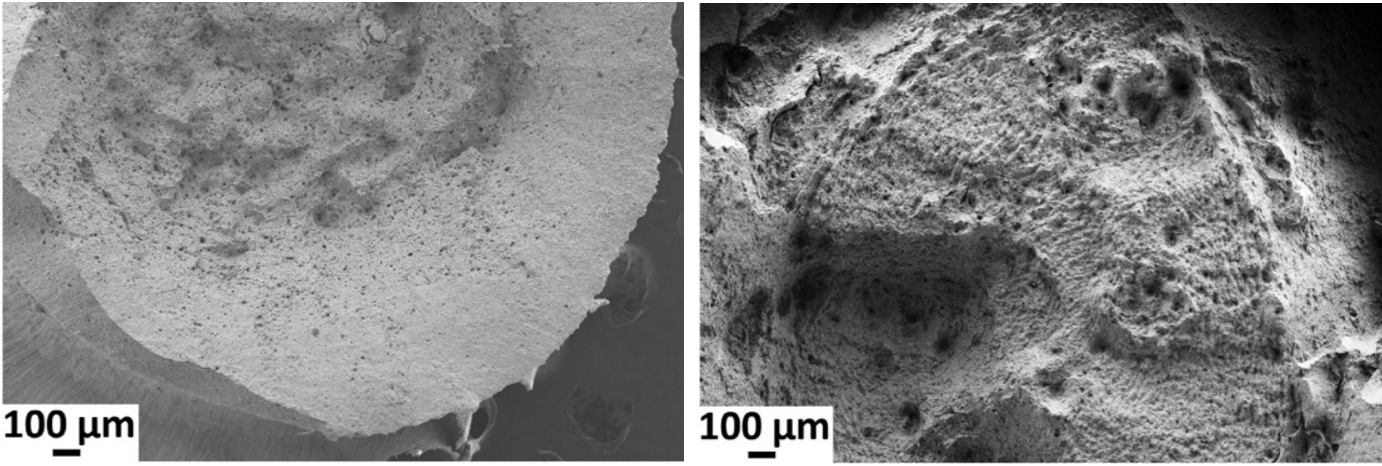
\includegraphics[width=0.7\linewidth]{Ch2/Figures/Wrought_vs_DMLS.PNG}}
    \caption{Comparison of wrought (left) and DMLS (right) test...Image adapted from \textit{A comparative study of microstructure and high-temperature mechanical properties of 15-5 PH stainless steel processed via additive manufacturing and traditional manufacturing}\cite{Roberts_Traditional_AM_15_5_testing}.} 
    \label{fig:2_Wrought_vs_DMLS_fracture surface}
\end{figure}
%


%Carlton et al. discovered SLM-printed stainless steel specimens with high porosity concentrations (> 2%) undergoing tensile testing fail in...under tension, while low porosity samples (< 1%) samples exhibit...failure (\ ....additionally, porosity increases.... [damage evolution and failure mechanisms...] as 

%-----------------------------------------------------------------------
\section{Warhead Performance \& Fragmentation Theories} \label{sec:2_Warhead_Fragmentation_Theories}
%-----------------------------------------------------------------------

A fragmenting warhead's effectiveness and lethality are primarily determined by the casing's material performance under the explosive loading. For instance, when a warhead detonates, the generated shock wave travels outward into the casing until reaching the casing's free surface with the atmosphere. At this point, a rarefaction (relief) wave reflects back into the casing until it reaches the inner wall surface, reflecting a shock wave back towards the outer surface. This wave reflection process continues to repeat, accelerating the casing outward, until the casing fractures \cite{Blast_injury_science_shockwave}. Since this creates an extremely fast and complex explosive event, experts continually try to simplify underlying physics using analytical expressions and models. One of the most widely used formulas for predicting a warhead's fragmentation velocity is the Gurney equation.  

%AM defects could impede the shockwave's transmission through the casing, decreasing it's overall contribution to material deformation.

%Voids may serve as local free surfaces, creating additional reflected waves within the casing itself.
%.....shockwaves accelerate

%Additive Manufacturing ductility comparison...fragment's accelerated 
%%%%%%%%%%%%%%%%%%%%%%%%%%%%%%%%%%%%
\subsection{Gurney Equation} \label{sec:2_Gurney}
%%%%%%%%%%%%%%%%%%%%%%%%%%%%%%%%%%%%
In the 1940s, R. W. Gurney researched fragmentation velocity of various military munitions at Ballistics Research Laboratories, located at Aberdeen Proving Grounds, MD.
Using a velocity camera positioned approximately 9 feet from the target, Gurney measured the initial fragment velocity of various types of explosive weapons. Gurney also employed a conservation of energy approach to mathematically characterize these detonations, concentrating on chemical-to-kinetic energy conversion to determine velocity of resulting fragments.

%Assumptions 
The kinetic energy $K$ of object $i$ is a function of its mass $m$ and velocity $V$, as shown in the fundamental equation below:
%Eq: Fundamental KE equation
\begin{equation}
K_{i} = \frac{1}{2}m_{i}{V_{i}}^2
\label{eq:2_KE}
\nomenclature{K}{Kinetic Energy}
\nomenclature{V}{Velocity}
\nomenclature{m}{Mass}
\end{equation}
%
Gurney hypothesized the amount of kinetic energy generated by detonating a unit mass of explosive is independent of projectile size; therefore, initial fragmentation velocity $V_0$ is not a function of the warhead's dimensions. Since detonations are dynamic events featuring multiple energy conversion stages over a short timespan, Gurney made several key assumptions to simplify the warhead detonation's underlying physics.

First, Gurney refined the conservation of energy principle and assumed all chemical energy provided by the explosive mass instantly converts to kinetic energy upon detonation, neglecting the work required to rupture the casing and all other energy conversion events occurring during the explosion. Therefore, the total amount of the energy per unit length of explosive is equal to the product of the explosive's specific energy $E$ and mass per unit length $C$. Since the casing and explosive masses both have kinetic energy after detonation, Gurney set the summation of these values equal to $EC$, as shown below: 
%Eq - Total KE in System 
\begin{equation}
EC = K_{Explosive} + K_{Casing}
\nomenclature{$E$}{Explosive Specific Energy}
\nomenclature{$C$}{Explosives Mass}
\label{eq:2_Overall_EC}
\end{equation}
%
where $K_{Explosive}$ and $K_{Casing}$ are the amounts of kinetic energy per unit length for the explosive and casing products, respectively. 

For the expanding detonation gases, Gurney assumed a uniform velocity distribution along the cylinder's entire length. This assumption is not valid in reality due to end effects, which are covered in further detail later in this section \cite{GurneyOriginal}. Additionally, Gurney assumed a linear velocity gradient in the radial direction, from the cylinder's centerline ($V_{r=0} = 0$) to its inner wall ($V_{r=a} = V_0$), as depicted in \cref{fig:2_Cylinder_V_r} below: 
%Fig - Velocity Gradient
\begin{figure}[H]
	\centering
 \fbox{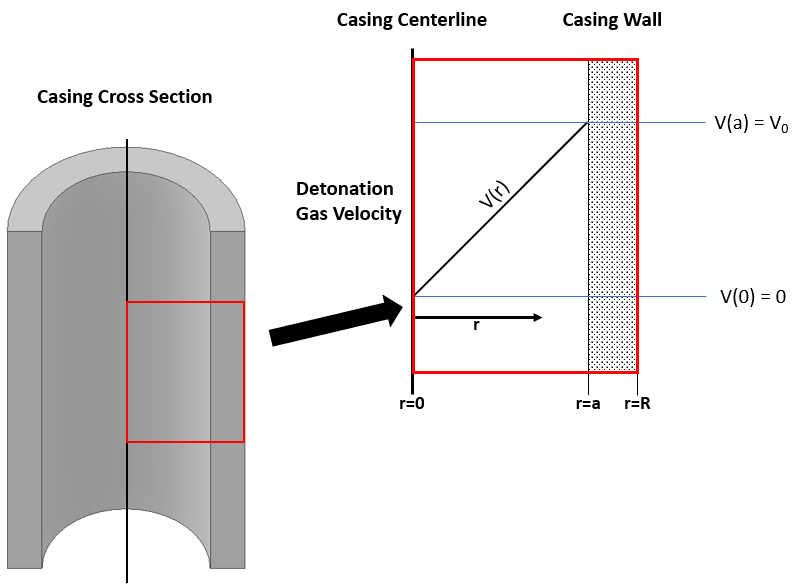
\includegraphics[width=0.7\linewidth]{Ch2/Figures/Cylinder_V_r.PNG}}
    \caption{Visual depiction of linear velocity gradient assumed by Gurney, 	based on an illustration from \textit{Gurney Energy of Explosives: Estimation of the Velocity and Impulse Imparted to Driven Metal} \cite{GurneyKennedy1970}}
	\label{fig:2_Cylinder_V_r}
\end{figure}
%
Consequently, the detonation velocity at any position within the casing is a function of distance from the cylinder's longitudinal axis, $r$,
%
\begin{equation}
V(r) = \frac{r}{a}V_0
\label{eq:2_linearvelocity}
\end{equation}
%

Another key assumption Gurney made was a constant density $\rho$ in the detonation product gases \cite{GurneyOriginal}. When the explosive is treated as a unit length cylinder with outer radius $a$ (casing inner radius), its density is then:
%Eq - Explosives density
\begin{equation}
\rho = \frac{C}{\pi{a^2}}
\label{eq:2_explosive_density}
\end{equation}
%
Furthermore, the volume $\volume$ for any portion of the unit length cylinder between $r$ and $r+dr$ (depicted in \Cref{fig:2_Cylinder_dr_calculation}) is: 
%Eq - Vol of cylinder portion
\begin{equation}
\volume = 2\pi{r}dr
\label{eq:2_unitcylindervolume}
\end{equation}
%
%Fig - Picture showing dr portion of explosive
\begin{figure}[H]
	\centering
 \fbox{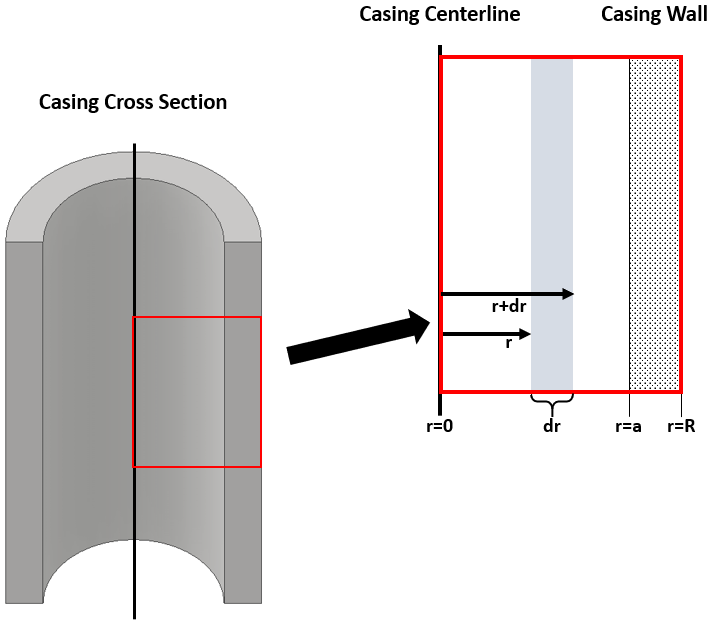
\includegraphics[width=.6\linewidth]{Ch2/Figures/Cylinder_dr_calculation.PNG}}
    \caption{Illustration portraying volume $\volume$ calculation in \Cref{eq:2_unitcylindervolume}, based on a drawing from \textit{ESTIMATION OF VELOCITY DISTRIBUTION OF FRAGMENTING WARHEADS USING A MODIFIED GURNEY METHOD} \cite{AFIT_Yves}}
\label{fig:2_Cylinder_dr_calculation}
\end{figure}
%
The explosive mass per unit length $C$ is determined by integrating \Cref{eq:2_unitcylindervolume} from the unit cylinder's center ($r = 0$), to its inner wall ($r = a$), and multiplying by $\rho$:
%
\begin{align}
C &= \rho\int_{0}^{a}\volume \nonumber \\
C &= \rho\int_{0}^{a}2\pi{r}dr
 \label{eq:2_Casingmassintegral}
\end{align}
%Eq -  KE Explosive Mass
Inserting \Cref{eq:2_linearvelocity,eq:2_Casingmassintegral} into  \Cref{eq:2_KE}, $K_{Explosive}$ becomes
\begin{align}
K_{Explosive} &= \frac{1}{2}CV(r)^2 \nonumber \\
&= \frac{1}{2} {\underbrace{\rho\int_{0}^{a}2\pi{r}dr}_\textrm{Mass term}}
{\underbrace{\vphantom{\int_{0}^{a}}\Big(\frac{r}{a}V_0\Big)^2}_\textrm{Velocity term}} \nonumber \\
 &= \rho\pi{V_0}^2\int_{0}^{a}\frac{r^3}{a^2}dr \nonumber \\
K_{Explosive} &= \frac{\rho\pi{V_0}^2{a^2}}{4}
\label{eq:2_K_explosive_density}
\end{align}
Using \Cref{eq:2_explosive_density}, \Cref{eq:2_K_explosive_density} is rewritten in terms of $C$:
%
\begin{align}
K_{explosive} &= \frac{C}{\pi{a}^2} \frac{\pi{V_0}^2{a^2}}{4} \nonumber \\
K_{explosive} &= \frac{C{V_0}^2}{4}\label{eq:2_K_explosive_mass} 
\end{align}
%
%Eq -  KE of Casing
Since Gurney assumed a constant fragmentation velocity $V_0$ in the metal cylinder, $K_{casing}$ is obtained using \Cref{eq:2_KE}  
\begin{equation}
K_{casing} = \frac{1}{2}M{V_0}^2
\label{eq:2_KE_casing}
\end{equation}
%
\Cref{eq:2_K_explosive_mass,eq:2_KE_casing} are inserted into \Cref{eq:2_Overall_EC}, relating the kinetic energy terms to the explosive's stored chemical energy. Rearranging variables results in \Cref{eq:2_finalGurney}, also known as the Gurney equation for cylindrical casings, 
%
\begin{align}
EC &= \underbrace{\frac{C{V_0}^2}{4}}_\textrm{$K_{Explosive}$}  + \underbrace{\frac{1}{2}M{V_0}^2}_\textrm{$K_{Casing}$} \nonumber \\
EC &= {V_{0}}^2\Big(\frac{C}{4} +\frac{M}{2} \Big) \nonumber \\
\frac{1}{V_{0}^2} &= \frac{1}{EC}  \Big(\frac{C+2M}{4} \Big) \nonumber \\
\frac{1}{V_{0}^2} &= \frac{1}{2E}  \Big(\frac{1}{2} + \frac{M}{C} \Big) \nonumber \\
{V_{0}^2} &= \frac{2E}{  \Big(\frac{1}{2} + \frac{M}{C} \Big)} \nonumber \\
{V_{0}^2} &= 2E\frac{\frac{C}{M}}{  \Big(1 + \frac{1}{2}\frac{C}{M} \Big)} \nonumber \\
{V_{0}} &= \sqrt{2E} \sqrt{\frac{\frac{C}{M}}{1 + \frac{1}{2}\frac{C}{M}}} 
\label{eq:2_finalGurney}
\nomenclature{$M$}{Casing Mass}
\nomenclature{$a$}{Cylinder Inner Radius}
\nomenclature{$R$}{Cylinder Outer Radius}
\nomenclature{$V_{0}$}{Initial Fragment Velocity}
\end{align}
%
where the Gurney Velocity Coefficient $\sqrt{2E}$ (or Gurney Constant) is calculated using the explosive's specific energy $E$, and has units of velocity. Additionally, \Cref{eq:2_finalGurney} features the explosive charge to metal mass ratio $C/M$, which is determined by casing dimensions and explosive density. Therefore, all variables in the Gurney equation are controlled by the experimental design, making it an effective comparison method for analyzing test results.  

Although the Gurney equation provides an uncomplicated method for calculating fragmentation velocity, it utilizes several assumptions which are not always practical in real world applications. For instance, since Gurney derived \Cref{eq:2_finalGurney} from a unit length cylinder, there is no way to incorporate the casing's length to diameter ratio $L/D$. Since Gurney's report was published, subsequent research revealed fragments formed around the ends of detonating cylindrical warheads with $L/D$ ratios $\leq$ 2 exhibited fragmentation velocities much lower than predicted by the Gurney equation \cite{AFIT_Yves}. This phenomenon is now referred to as ``end effects."
\nomenclature{L/D}{length to diameter ratio}

End effects occur due to interactions between shock waves and rarefaction (relief) waves. Warheads are commonly designed with a single detonator located at one end of the cylinder. When the cylinder is detonated, shock waves develop and propagate away from the detonator location. Upon reaching the free surface between the casing and surrounding environment (air), rarefaction (relief) waves form, reflecting back into the casing and detonating explosive. Since a rarefaction wave lowers the pressure of the substance it travels through, it decreases the amount of loading available to expand the casing outward, inevitability lowering the fragmentation velocity.

Since the detonation is not instantaneous, it takes a finite amount of time for the chemical reaction process to travel down the entire length of the explosive filling. As a result, fragments located near the detonation end of the cylinder form rarefaction (relief) waves as the explosive is detonating, resulting in lower local fragment velocities. Analytical modeling of exploding TNT-filled cylinders in \textit{A Parametric Investigation and Optimization of a Cylindrical Explosive Charge}, illustrated in \cref{fig:2_Sawtooth_waves}: 
%Figure showing detonation/rarefaction wave interaction
\begin{figure}[H]
	\centering
 \fbox{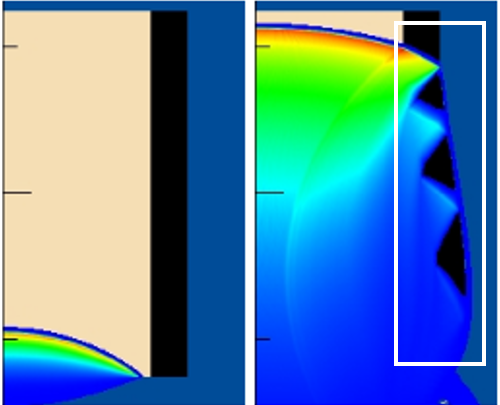
\includegraphics[width=0.6\linewidth]{Ch2/Figures/Beaver_End_Effects.PNG}}
    \caption{Two images depicting the evolution of a detonation wave in TNT (tan region), where the white box indicates the rarefaction/detonation wave interaction region .Image adapted from \textit{A Parametric Investigation and Optimization of a Cylindrical Explosive Charge} \cite{MarquetteEndEffects}.}
	\label{fig:2_Sawtooth_waves}
\end{figure}
%
Additionally, the shock wave generated by the detonator travels through the explosive filling and reaches the opposite end of the cylinder before the chemical reaction process is complete, creating more rarefaction waves at the far end's free surface. Consequently, in cylindrical warheads with low $L/D$ values, reduced fragmentation velocities also occur at the opposite end of the detonator \cite{AFIT_Yves,MarquetteEndEffects}. This phenomenon manifested in experiments conducted by Huang and Feng, where a cylinder with $L/D$ = 1.3 was detonated, producing the fragmentation velocity profile shown in \Cref{fig:2_end_effects} below \cite{HuangEndEffects}:    
%Figure showing impact of end effects on fragmentation velocity
\begin{figure}[H]
	\centering
 \fbox{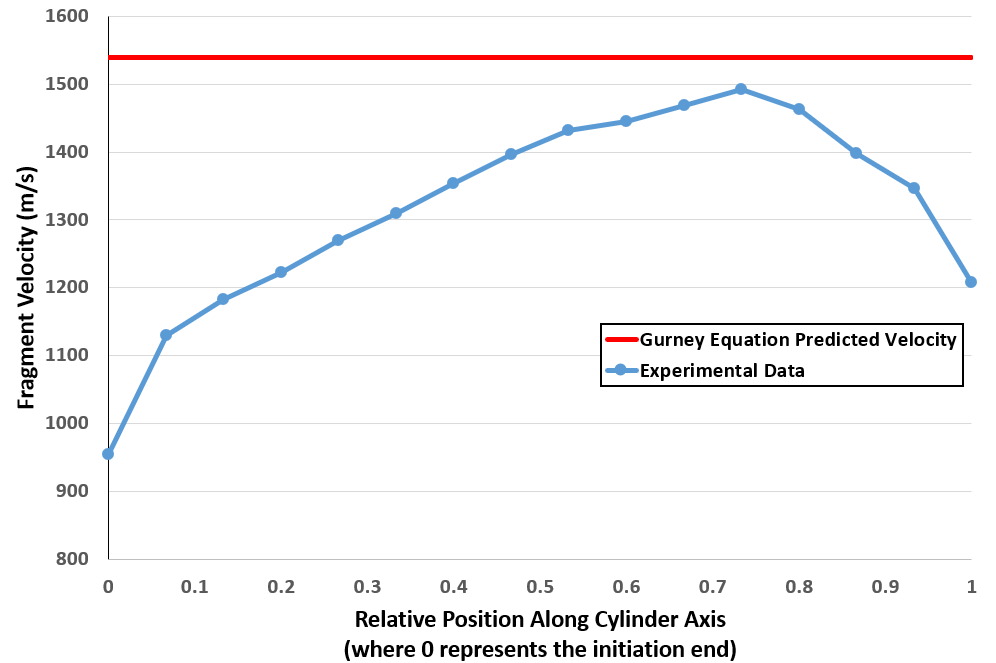
\includegraphics[width=0.7\linewidth]{Ch2/Figures/End_Effects.PNG}}
    \caption{Experimental data from \textit{Axial distribution of Fragment Velocities from cylindrical casing under explosive loading} showing the influence of end effects during fragmentation events \cite{HuangEndEffects}.}
	\label{fig:2_end_effects}
\end{figure}
%
\cref{fig:2_end_effects} compares Huang and Feng's measured data with the corresponding Gurney equation prediction. Near the initiation end (0 on the horizontal axis), shock and relief wave interactions (as shown in \cref{fig:2_Sawtooth_waves}) result in fragmentation velocities significantly lower than predicted by the Gurney equation. Similarly, the rarefaction waves formed after the initial detonation wave reaches the cylinder's far end (1 on the horizontal axis) weaken the local pressure loadings generated by the ongoing explosive filling detonation, reducing far end casing expansion rates and the resulting fragmentation velocities.

%Gurney equation doesn't account for material properties
Another Gurney equation limitation is its inability to account for casing material properties. 
%%%% Include copper steel graph

%and concluded the initial detonation wave notably contributes to casing acceleration. 
\cite{WangDuctilityExpansion}


In addition to fragmentation velocity, weapons developers also use fragment mass distribution to characterize the potential damage caused by exploding warheads. Some weapons even feature ``pre-fragmented" designs, controlling the resulting fragments' size and shape \cite{DrielsWeaponeering}. While many fragmentation studies have transitioned to computer-based modeling to exploit high performance computer capabilities \cite{GrisaroFragmentVelocityDistribution,MarquetteEndEffects,MoxnesRingFragmentationSimulation}, most researched is derived from N.F. Mott's fragmentation theory. 
%%%%%%%%%%%%%%%%%%%%%%%%%%%%%%%%%%%%
\subsection{Mott Fragmentation Model}
%%%%%%%%%%%%%%%%%%%%%%%%%%%%%%%%%%%%

%Due to the layering scheme present in AM,....Mott fragmentation distribution cannot be applied from a length perspective


In early 1940s England, N.F. Mott began studying warhead fragmentation to support the ongoing World War II effort. Through a series of reports, Mott attempted to model the weight distribution of fragments created by exploding bombs and shells. In 1943, he developed two scaling relations for fragmenting cylindrical shells, giving weapons developers the ability to study the effects of modifying warhead dimensions without conducting experimental tests \cite{GradyMottLegacy}.     
The following distribution predicts the number of fragments $n(m)$ with weights between $m$ and $m + dm$: 
%
\begin{equation} %page 141,228 - Grady ; Fragmentation of HE Shells
	dN = B\exp\bigg({-\frac{\sqrt{m}}{M_{A}}}\bigg)d\sqrt{m}
    \label{eq:2_Mott1943_dN}
\end{equation}
%
where $M_{A}$ is defined as
%
\begin{equation} 
	M_{A} = {\Gamma}t^{\nicefrac{5}{6}}d_{in}^{\nicefrac{1}{3}}\Big(1+\frac{t}{d_{in}}\Big) 
    \label{eq:2_Mott1943Ma}
\end{equation}
%
In \Cref{eq:2_Mott1943_dN,eq:2_Mott1943Ma}, $m$ is the fragment mass, $B$ is a distribution factor, and $\Gamma$ is an empirical constant based on explosive properties, and $d_{in}$ and $t$ are the casing's inner diameter and thickness, respectively. Next, fragment mass distribution $dM$ is obtained by multiplying \Cref{eq:2_Mott1943_dN} by $m$:
%Eq:dM - ma
\begin{align}
dM &= mdN \nonumber \\
dM &= mB\exp\bigg({-\frac{\sqrt{m}}{M_{A}}}\bigg)d\sqrt{m}
 \label{eq:2_Mott1934_dM}
\end{align}
%
Since the sum of the fragment masses is equal to the casing mass $M$, $B$ is calculated using integration by parts $\int{udv} = uv - \int{vdu}$: 
%Eq - B Derivation
\begin{align}
M &= \int_{0}^{\infty}dM \nonumber \\
 &= B\int_{0}^{\infty}m\exp\bigg({-\frac{\sqrt{m}}{M_{A}}}\bigg)d\sqrt{m}
\nonumber \\
 &= B\int_{0}^{\infty}x^{2}e^{-\tfrac{x}{y}}dx \text{\phantom{..............} where $x = \sqrt{m}$ and $y = M_{A}$} 
\nonumber \\ 
 &= B\bigg[-ye^{-\tfrac{x}{y}}x^2+\int{2y}e^{-\tfrac{x}{y}}xdx\Bigg]_{0}^\infty \nonumber \\
 &= B\bigg[-ye^{-\tfrac{x}{y}}x^2+{2y}\Big(-ye^{-\tfrac{x}{y}}x+\int{ye^{-\tfrac{x}{y}}}dx\Big)\Bigg]_{0}^\infty \nonumber \\
 &= B\bigg[-ye^{-\tfrac{x}{y}}x^2+{2y}\Big(-ye^{-\tfrac{x}{y}}x-{y^2e^{-\tfrac{x}{y}}}\Big)\Bigg]_{0}^\infty \nonumber \\
 &= B(0-(-2y^3)) \nonumber \\
M &= 2B{M_{A}}^3 \nonumber \\
B &= \frac{M_0}{2{M_{A}}^3}
\label{eq:2_Mott1934_B}  
\end{align}
%
Mott's cumulative fragment distribution is obtained by integrating \Cref{eq:2_Mott1943_dN} and substituting in \Cref{eq:2_Mott1934_B} to incorporate material properties:
%Eq - Cumulative Fragment Distribution
\begin{align}
N(m) &= \int_{m}^{\infty}dN \nonumber \\
 &= B\int_{m}^{\infty}\exp\bigg({-\frac{\sqrt{m}}{M_{A}}}\bigg)d\sqrt{m} \nonumber \\
&= \frac{M_0}{2{M_{A}}^3}\int_{m}^{\infty}\exp\bigg(-{\frac{\sqrt{m}}{M_{A}}}\bigg)d\sqrt{m}
\nonumber \\
&= \frac{M_0}{2{M_{A}}^3}\bigg[-M_{A}\exp\bigg(-\frac{\sqrt{m}}{M_{A}}\bigg) \bigg]_{m}^\infty  \nonumber \\
&= \frac{M_0}{2{M_{A}}^3}\bigg(0 - \bigg(-M_{A}\exp\bigg(-\frac{\sqrt{m}}{M_{A}}\bigg)\bigg) \bigg)  \nonumber \\
N(m) &= \frac{M_0}{2{M_{A}}^2}\exp\bigg(-\frac{\sqrt{m}}{M_{A}}\bigg)
\label{eq:2_Mott1934_Cumulative_frag}  
\end{align}
%
where $N(m)$ is the number of resulting fragments with a mass greater than $m$.

In \textit{Fragmentation of shell cases}, Mott noted exploding forged steel shells typically fracture in segments running parallel to the casing's longitudinal axis, forming large, thin fragments \cite{Mott1947}. This is likely due to the largely homogeneous composition found in conventionally produced metals, meaning the casing does not have any substantial weak points prone to early failure. By contrast, the additively manufactured metals featured in this research have inherent flaws by nature of the manufacturing process (as covered in \Cref{sec:2_SLM_drawbacks}). The use of a layering construction process and localized heat source in \gls{DMLS} creates a non-uniform distribution of internal features (micropores, melt pool boundaries, etc.) along the part's build direction. As shock waves and detonation product gases exert loadings on these weakened imperfections, they may prematurely fracture, causing the cylinder casing to fail.

Similar to the Gurney equation, the Mott fragmentation model also lacks a variable to readily account for the casing's material properties. 
 In Mott's original work, the munitions' mild steel casings properties were incorporated into empirically derived $\Gamma$ values \cite{Mott_Fragmentation_DOE}. While this was largely sufficient for predicting fragmentation characteristics of weapons used during the 1940s, there is no empirical solution for the wide array of materials featured in modern weapons.
 Although the fragmentation theories presented in \Cref{sec:2_Warhead_Fragmentation_Theories} are extremely useful analytical tools, experimental testing is still an essential element of weapons design. Unfortunately, explosives testing features extremely fast detonation rates are not observable to the naked eye and common optical equipment. Therefore, to maximize data collected during testing, specialized diagnostic methods are used to witness the entire process.   

%-----------------------------------------------------------------------
\section{Diagnostic Techniques} \label{sec:2_Diagnostic_Techniques}
%-----------------------------------------------------------------------


%%%%%%%%%%%%%%%%%%%%%%%%%%%%%%%%%%%%
\subsection{High Speed Photography} \label{sec:2_Diagnostic_Photography}
%%%%%%%%%%%%%%%%%%%%%%%%%%%%%%%%%%%%

Since explosions involve extremely fast chemical reaction rates (typical detonation velocities in air are 5-10 km/s) \cite{Cooper1996}, cylinder casing fractures occurs within tens of microseconds of detonation \cite{ExpandingFractureBehavior1045Cylinder}.
%, if visual investigations are desired.
%Historical high speed photography relied on…
%Modern high speed cameras store….directly on, enabling frame rates of X million \gls{fps}
Fortunately, modern high speed cameras store….directly on, enabling frame rates on the order of millions of \gls{fps}. Unlike other high speed recording techniques, such as \gls{DPV} and Flash Radiograph, which involve complex, specialized support equipment, high speed cameras only require a calibrated lighting source and computer interface for camera synchronization.   
%. While these methods can achieve...(very accurate results?), they are typically limited to analyzing...(one surface?) and require specialized test equipment. For instance, 

%%%%%%%%%%%%%%%%%%%%%%%%%%%%%%%%%%%%
\subsection{\glsentryfull{DIC}} \label{sec:2_Diagnostic_DIC}
%%%%%%%%%%%%%%%%%%%%%%%%%%%%%%%%%%%%
\gls{DIC} is a non-contact optical tracking method used to capture the deformation and displacement of materials in motion. This is accomplished by comparing the movement of small pixel groups ``subsets" over a series of images. Since the software's accuracy is determined by its ability to identify and trace pixel movements, both the test specimen and its surrounding environment must be specially prepared for optimal data collection conditions. This is typically done by coating a portion of the test specimen with a speckle pattern for the \gls{DIC} software to identify and track.

Over the past 20 to 25 years, \gls{DIC} has emerged as a reliable method for quantifying strains and deformations observed during material testing. Originally used to monitor quasi-static deformations at low imaging rates (5-15 \gls{fps}), it is now used regularly in explosive applications. Additionally, \gls{DIC} allows for localized displacement measurements, which is advantageous for analyzing materials with non-homogeneous grain structures \cite{ReuDICapplication}.  %the application of high speed DIC

While only one camera is needed for 2D strain and deformation measurements, the use of two cameras, also known as a stereo system configuration, allows for 3D \gls{DIC} analysis \cite{ArtandApplicationDICReu}. An example \gls{DIC} stereo system setup for fragmentation testing is illustrated in \Cref{fig:2_DIC_setup} below:  
%
\begin{figure}[H]
	\centering
 \fbox{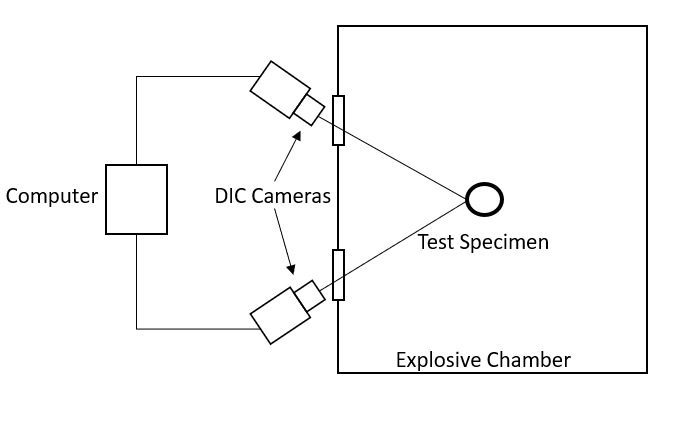
\includegraphics[width=0.7\linewidth]{Ch2/Figures/DIC_Figure.PNG}}
    \caption{Example \gls{DIC} Setup, based on illustrations from \textit{Observations in Explosive Systems with High-Speed Digital Image Correlation} \cite{DICimageObservations}}
	\label{fig:2_DIC_setup}
\end{figure}
%
%\gls{DIC} analysis begins by first calibrating the cameras to the test setup,

%DIC software overlays a colorized heat map to depict deformation at any point within the selected region of interest

%%%%%%%%%%%%%%%%%%%%%%%%%%%%%%%%%%%%
\subsection{Fragment Tracking} \label{sec:2_Fragment_tracking}
%%%%%%%%%%%%%%%%%%%%%%%%%%%%%%%%%%%%

Another useful diagnostic technique is the Matlab-based fragment tracking software developed by Daniel Guildenbecher from \gls{SNL}.


%
%-----------------------------------------------------------------------
\section{Summary} \label{sec:2_Summary}
%-----------------------------------------------------------------------
Chapter II provides a brief overview of military weaponeering limitations and how \gls{AM} presents a novel approach to custom building munitions for specific targets. It details \gls{PBF} processing and resulting material characteristics and fragmentation theories describing casing failure in explosive environments. Additionally, this chapter outlines the importance of high speed photography for investigating explosive events, and how \gls{DIC} extracts mechanical properties of test subjects. 
While experts continually look for techniques to increase weapons effectiveness while decreasing collateral damage, there is little research incorporating additively manufactured metals into explosive applications. This thesis characterizes the behavior of \gls{AM}-printed metal casings under explosive loadings, compares performance with classic fragmentation models used in weapons research, and calculates mechanical properties using visual tracking techniques.

%--------%%%%%%%------%%%%%%
%Given the previous research, I need to address...
%I will perform my research by..... (Detonating cylinders)
%I will quantify my experiments by.....

%Building on Gurney's research methodology, $L/D$ ratio was varied in the \gls{AM}-printed casings' design to induce multiple $C/M$ [data points]?? 


%Before additively manufactured metals are utilized in explosive applications, their....need to....

%This research will address by detonating.....

%DIC analysis will extract deformation and fragmentation velocities....

%This research uses fragmentation models developed by Gurney and Mott as a foundation to characterize the performance of exploding additively manufactured casings. 

	\chapter{Methodology} \label{chap:3}

%-----------------------------------------------------------------------
%\section{Objective}
%-----------------------------------------------------------------------
This research investigated the behavior of additively manufactured cylindrical casings subjected to internal explosive loadings. Test samples were constructed using \gls{PBF} and filled with a controlled amount of explosives. The specimens were detonated inside indoor chambers while high speed cameras observed and recorded the detonation events. Fragmentation velocities and corresponding mechanical properties of the 15-5PH \gls{PBF}-printed stainless steel samples were derived from the captured images through \gls{DIC} analysis. Fragments formed during the detonation event were weighed to compare experimental results with classic fragment mass distribution models.

% %-----------------------------------------------------------------------
% \section{Theory}
% \label{sec:3_Theory}
% %-----------------------------------------------------------------------
% When an explosives-filled cylindrical casing is detonated, it's walls undergo rapid expansion before ultimately fracturing and
% The casing's material and mechanical properties determine its ability to elongate and withstand fracture during an explosion.

%-----------------------------------------------------------------------
\section{Specimen Design} \label{sec:3_specimen}
%-----------------------------------------------------------------------



Test samples were constructed via \gls{PBF} using 15-5PH stainless steel powder feedstock. \gls{PBF} was selected because of its ability to fabricate metal parts with mechanical properties suitable for high temperature environments. Additionally, 15-5PH stainless steel was chosen to synchronize this research with other ongoing \gls{DoD}-sponsored \gls{AM} projects, in addition to its favorable mechanical properties \cite{AFIT_Dempsey, EOS_StainlessSteel_M290}. The \gls{PBF} technique employed in this research was \gls{DLMS}.

\gls{DMLS} test specimens were manufactured by 3Diligent in El Segundo, California and by i3D MFG, located in Bend, Oregon.
3Diligent samples were constructed using an EOS \gls{DMLS} system (exact model considered proprietary information) and i3D MFG specimens were fabricated using EOS's EOSINT M 280 system. Both companies used EOS's StainlessSteel PH1 feedstock, a 15-5PH stainless steel powder featuring the chemical composition given below in \cref{tab:3Diligent_Chem_Comp}:

% Tab - 3Diligent Material Composition
\FloatBarrier
\begin{table}[h]
  \centering
  \caption{Chemical composition of 15-5 PH Stainless Steel feedstock used by 3Diligent and i3D MFG for \gls{DMLS} cylinder printing  \cite{EOS_StainlessSteel_M290}}
    \begin{tabular}{lc}
    \multicolumn{2}{c}{\textbf{\large EOS StainlessSteel PH1}} \\
    \midrule
    \multicolumn{1}{c}{\textbf{Element}} & \textbf{Percentage (weight)} \\
    \midrule
    Iron (Fe) & (balance) \\
    Chrormium (Cr) & 14.0 - 15.5 \\
    Nickel (Ni) & 3.5 - 5.5  \\
    Copper (Cu) & 2.5 - 4.5 \\
    Manganese (Mn) & 1.00 \\
    Silicon (Si) & 1.00 \\
    Carbon (C) & 0.07 \\
    Molybdenum (Mo) & 0.5 \\
    Niobium (Nb) & 0.15 - 0.45 \\
    \bottomrule
    \end{tabular}%
    \label{tab:3Diligent_Chem_Comp}%
\end{table}
\FloatBarrier
Following construction and a post-processing precipitation hardening treatment of 480\degree C for 4 hours, room temperature tensile testing of EOS's StainlessSteel PH1 in accordance with ISO 6892:1998(E) Annex C yields the following mechanical properties:

% Table generated by Excel2LaTeX from sheet '3Diligent'
\begin{table}[htbp]
  \centering
  \caption{3Diligent's 15-5 PH stainless steel mechanical properties \cite{EOS_StainlessSteel_M290}}
    \begin{tabular}{lc}
    \multicolumn{2}{c}{\textbf{\large EOS StainlessSteel PH1}} \\ 
    \midrule
    %
    \multicolumn{2}{l}{\textbf{Ultimate Tensile Strength (MPa)}} \\
    Longitudinal & 1440 $\pm$ 100 \\
    Transverse  & 1450 $\pm$ 100 \\[1 ex]
    %
    \multicolumn{2}{l}{\textbf{Yield Strength (MPa)}} \\
    Longitudinal & 1350 $\pm$ 100 \\
    Transverse & 1300 $\pm$ 100 \\[1 ex]
    %
    \multicolumn{2}{l}{\textbf{Elongation at Failure (\%)}} \\
    %\midrule
    Longitudinal & 13 $\pm$ 3 \\
    Transverse  & 15 $\pm$ 3 \\
    \bottomrule
    \end{tabular}%
  \label{tab:addlabel}%
\end{table}%
Components produced using EOS's StainlessSteel PH1 powder and M 290 printer have a density of approximately 7.7 g/cm$^{3}$ (compared to a $\sim$7.8 g/cm$^{3}$ density exhibited by conventional 15-5 PH stainless steel H900 \cite{AKSteel_Conventional_SS}) and a 20 $\mu$m layer thickness \cite{EOS_StainlessSteel_M290}.

%%%%%%% i3D MFG Section %%%%%%%%
\gls{DMLS}-printed casings were constructed by Oregon-based i3D MFG using EOS's StainlessSteel PH1 powder (\label{tab:3Diligent_Chem_Comp}) and M 290 printer



...The material composition of 15-5 PH Stainless Steel used by i3D MFG is shown in   




%Thirty specimens were fabricated for each of the three models, totaling 90 test samples for the experiment. 
%In total, x samples were detonated...


%%%%%%%%%%%%%%%%%%%%%%%%%%%%%%%%%%%%
\subsection{Specimen Dimensions} \label{sec:3_specimen_dimensions}
%%%%%%%%%%%%%%%%%%%%%%%%%%%%%%%%%%%%

Due to budget and time constraints, small-scale test samples ($C <$ 1 g) were used to maximize the amount of data collected during the allocated test window. Researchers at \gls{SNL} discovered fragmentation properties of metallic casings undergoing explosive loading remain largely unchanged when scaled down appropriately (private communication). This significantly reduces experimental preparation and completion times, allowing for more detonation events in a given time frame. 

In order to capture the effects of varying the explosive to casing mass ratio $C/M$, three different casing \gls{CAD} models were built, each having a unique outer diameter $d_{outer}$. By holding all other dimensions constant, this produced a variation in casing mass $M$, and thus different $C/M$ values, producing the experiment's control variable. An example \gls{CAD} model is shown in \Cref{fig:3_Casing_CAD_model}, and \Cref{fig:3_Casing_dimensions} compares the three models' dimensions. Both manufacturers received the same \gls{CAD} models to minimize variation in the test specimens.

%Fig - An example showing one of the CAD models
\begin{figure}[H]
	\centering
 \fbox{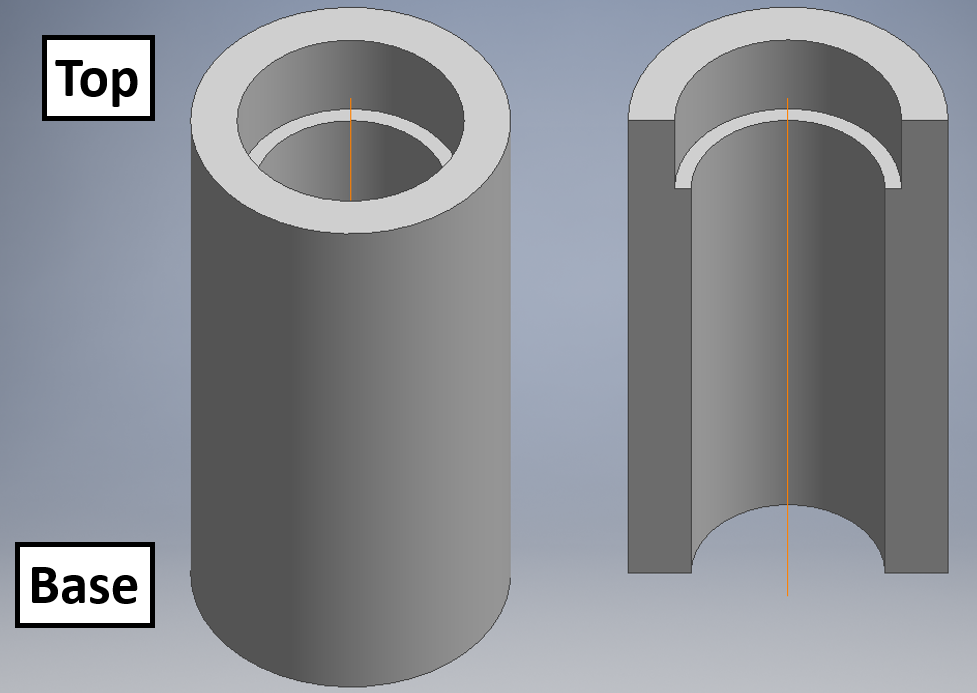
\includegraphics[width=0.6\linewidth]{Ch3/Figures/Example_CAD_Model.PNG}}
    \caption{Example casing \gls{CAD} model}
	\label{fig:3_Casing_CAD_model}
\end{figure}
%
%
\begin{figure}[H]
	\centering
 \fbox{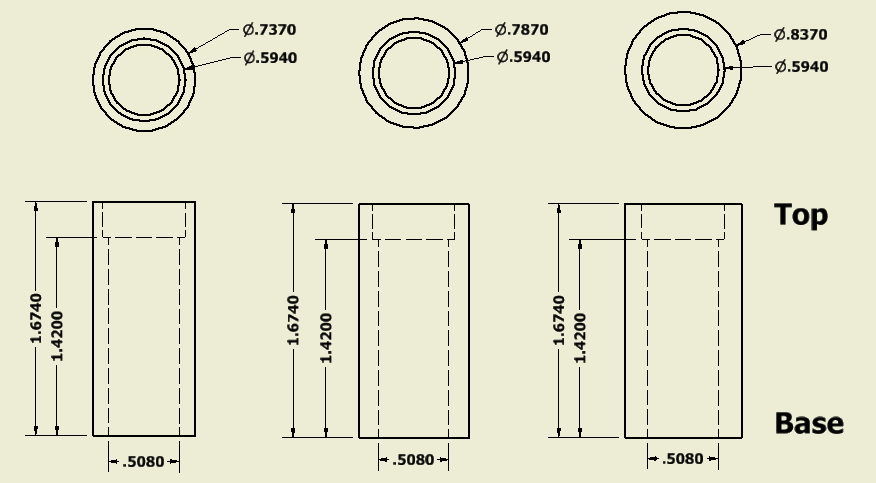
\includegraphics[width=1.0\linewidth]{Ch3/Figures/CAD_Model_Comparison.PNG}}
    \caption{Dimensions of the three test specimens used in this research (all dimension values in cm)}
	\label{fig:3_Casing_dimensions}
\end{figure}
%

%%%%%%%%%%%%%%%%%%%%%%%%%%%%%%%%%%%%
\subsection{RP-80 Detonator} \label{sec:3_RP80}
%%%%%%%%%%%%%%%%%%%%%%%%%%%%%%%%%%%%
Detonators are traditionally used to initiate an explosion of a larger mass of explosives; however, \gls{SNL} converted Teledyne RISI's RP-80 exploding bridgewire detonator (\Cref{fig:3_RP-80_Layout}) into a ``surrogate" explosive device for sub-scale fragmentation testing. This is accomplished by replacing the RP-80's explosive train casing with the test specimen, creating a standalone explosive with the RP-80's internal 0.203 g of explosive filling. %Reword? 

%insert two figures, overall rp-80, and outer casing
%by fitting sleeves around the detonator's internal explosives.

%Fig - RP-80 design with cross section showing the explosive train's internal components
\begin{figure}[H]
	\centering
 \fbox{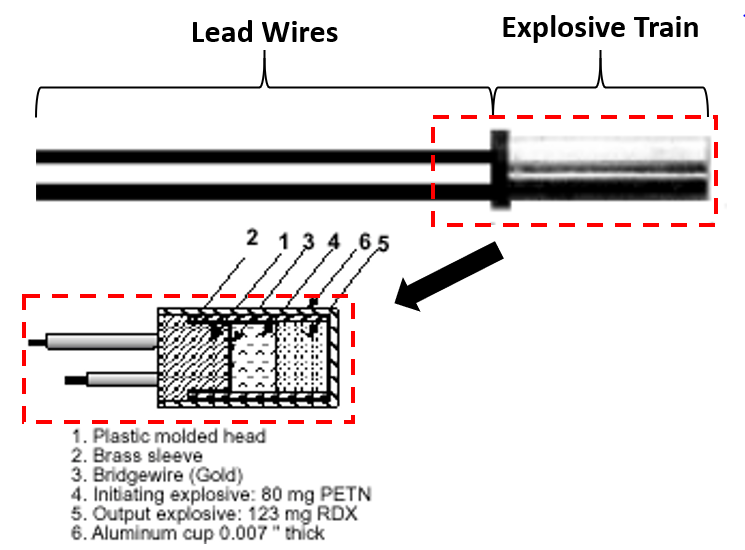
\includegraphics[width=0.6\linewidth]{Ch3/Figures/RP-80_Layout.PNG}}
    \caption{RP-80 detonator design, with a cross section adapted from Teledyne RISI's website illustration\cite{TeledyneRP-80}}
	\label{fig:3_RP-80_Layout}
\end{figure}
%
%Furthermore, by replacing the manufacturer's original outer sleeve with the test cylinder 
%commercial detonators are provide sufficient explosive filling (Private communication).    
%employed in this research, using an RP-80 detonator as the explosive filling.


%%%%%%%%%%%%%%%%%%%%%%%%%%%%%%%%%%%%
\subsection{Sample Manufacturing \& Preparation} \label{sec:3_Sample_Manufacturing}
%%%%%%%%%%%%%%%%%%%%%%%%%%%%%%%%%%%%
\begin{spacing}{1}
\noindent
\textbf{\textit{(rough draft note: Additional manufacturing details and images will be added once test specimens are constructed )}}
\end{spacing}
\vspace{1cm}

Test sample \gls{CAD} models were designed in Autodesk Inventor and then converted into STEP files for \gls{SLM} machine compatibility. These files were provided to I3DMFG...

After manufacturing was complete, 0.200 cm of length was removed from cylinders' bases via Wire \gls{EDM} to compensate for build plate effects generated during \gls{DMLS}, yielding an overall length of 1.474 cm for all test specimens. 

Test samples were filled with ...g of \gls{PETN} by explosives experts from \gls{SNL} and bored to remove any variations resulting from \gls{DMLS} processing.

Furthermore, \gls{AM}-printed 15-5PH stainless steel has exhibited tensile properties comparable to wrought and cast metals in previous research, further increasing its... 

%Paragraph on how Dan uses RP-80 for subscale testing of material fragmentation behavior, need to source this

%The RP-80 is an electronic bridgewire detonator used

%\ref{method_RP-80}
%Due to its design, the RP-80 detonator samples were limited to a L/D ratio of xx or lower. Consequently,....end effects 
%The sleeve's inner diameter was held constant to...
%By varying outer diameter and length within allowable limits, sleeves were constructed...  

%-----------------------------------------------------------------------
\section{Data Collection System} \label{sec:3_specimen}
%-----------------------------------------------------------------------

Two Shimadzu HPV-X2 high speed cameras were used to capture the detonation events using a [number] \gls{fps} frame rate..... This stereo camera configuration enables three-dimensional material displacement and deformation measurements during the subsequent \gls{DIC} analysis (\Cref{sec:3_digital_image_correlation}).  The cameras were mounted on sliding brackets .... 

For each test event, 128 images were recorded and stored on the cameras' onboard memory system, using a signal from the... to trigger the recording.


Two laser light sources, Cavitar's CAVILUX Smart and Specialised Imaging's SI-LUX640, were used to illuminate the detonation events. These systems were configured to emit 640 nm wavelength pulsed laser light and synchronized with the selected camera frame rate. To minimize the amount of background and detonation-generated light reaching the lenses and infiltrating the recorded images, both cameras were fitted with optical filters, restricting allowable light transmission to 640 $\pm$ 10 nm wavelengths.  


%In order to optimize high speed camera.... while.... minimize the influence of unwanted light sources,


%-----------------------------------------------------------------------
\section{Experimental Procedure} \label{sec:experimental_procedure}
%---------------------------------------------------
To maximize the amount and breadth of data collected


%%%%%%%%%%%%%%%%%%%%%%%%%%%%%%%%%%%%
\subsection{Overall Field of View } \label{sec:3_specimen_dimensions}
%%%%%%%%%%%%%%%%%%%%%%%%%%%%%%%%%%%%
The first three detonations focused on characterizing overall cylinder behavior 


%First, a large field of view test was performed to determine the optimal size window for \gls{DIC} data collection 



Test samples were detonated inside \gls{SNL}'s [specific chamber name] indoor explosives chambers. High speed cameras were positioned outside of the chambers....Following test completion, the captured images were exported to the computer system for follow-on \gls{DIC} analysis.
%-----------------------------------------------------------------------
\section{\glsentryfull{DIC} Analysis} \label{sec:3_digital_image_correlation}
%-----------------------------------------------------------------------
\begin{spacing}{1}
\noindent
\textbf{\textit{(rough draft note: This section will be completed after performing the experimental testing and \gls{DIC} analysis)}}
\end{spacing}
\vspace{1cm}


\gls{DIC} analysis was performed using \gls{SNL}'s DICe software package....

%and \gls{SNL}'s DICe software package was used for \gls{DIC} analysis. \cite{ReuDICapplication}

%-----------------------------------------------------------------------
\section{Fragment Mass Measurements}
\label{sec:3_digital_image_correlation}
%-----------------------------------------------------------------------
\begin{spacing}{1}
\noindent
\textbf{\textit{(rough draft note: This section will be completed after performing experimental mass measurements)}}
\end{spacing}
\vspace{1cm}


Fragment masses were measured using....This scale has a tolerance of...After all measured values were recorded,....

%-----------------------------------------------------------------------
\section{Summary} \label{sec:3_summary}
%-----------------------------------------------------------------------
Chapter 3 details the experimental approach used to study and characterize fragmentation properties of explosives-filled additively manufactured cylinders. Test samples designed in Autodesk Inventor software were fabricated via \gls{DMLS}. After filling the specimens with explosives, detonations were performed inside indoor blast chambers with high speed cameras monitoring casing expansion and fragmentation. After data collection was concluded, fragmentation properties were computed using \gls{DIC} analysis and fragment mass measurements.



%	\chapter{Results and Analysis}
\label{chap:4}

%-----------------------------------------------------------------------
%Chapter 4 Findings and Results
%-----------------------------------------------------------------------

% Nomenclature for Chapter 4

% Acronyms for Chapter 4
%	\newacronym{psd}{PSD}{Power Spectral Density}
%	\newacronym{fea}{FEA}{Finite Element Analysis}
%	\newacronym{vf}{VF}{Volume Fraction}
%	\newacronym{naca}{NACA}{National Aviation Commission Advisory}
%	\newacronym{fem}{FEM}{Finite Element Model}
%	\newacronym{leo}{LEO}{Low-Earth Orbit}

%-----------------------------------------------------------------------
\section{Chapter Overview}
%-----------------------------------------------------------------------



\begin{equation}
\label{e:Drag_Force}
F_{d}=\frac{1}{2}C_{d}A\rho v^2
\end{equation}
\nomenclature{$C_{d}$}{Coefficient of drag}
\nomenclature{$A$}{Area of solar panel}
\nomenclature{$\rho$}{Atmospheric density}
\nomenclature{$v$}{Speed of the satellite}

where $C_{d}$ is the drag coefficient, A is the area of solar panel projected in the velocity direction, $\rho$ is the atmospheric density, and $v$ is the speed of the satellite. For a simple approximation it is safe to assume an exponential model for atmospheric density shown in Equation \ref{e:atm}, and a circular orbit which yields Equation \ref{e:Orbital_Vel}:

\begin{equation}
\label{e:atm}
\rho=\rho_o e^{-h/H}
\end{equation}
\nomenclature{$\rho_o$}{Atmospheric density at sea level}
\nomenclature{$h$}{Orbital altitude}
\nomenclature{$H$}{Atmospheric scale height}

\begin{equation}
\label{e:Orbital_Vel}
v=\sqrt[]{\frac{\mu}{r}}
\end{equation}
\nomenclature{$\mu$}{Earth's gravitational parameter}
\nomenclature{$r$}{Orbital radius}

where $\rho_o$ is the representative atmospheric density at sea level, $h$ is the orbital altitude, and $H$ is the Atmospheric Scale Height, which ranges from 6 km to 8 km, and for the purposes of a realistic approximation, 7 km was chosen. In Equation \ref{e:Orbital_Vel}, $v$ is orbital speed, $\mu$ is Earth's Gravitational Parameter, and $r$ is the orbital radius, which is Earth's radius plus the orbital altitude \cite{wiesel2010spaceflight}.

Picking a representative orbital altitude of $r=500$ km, and using constant values of $\mu=398\:601$ km$^3$/s$^2$ and $\rho_o=1.225$ kg/m$^3$, the air density at altitude 
%-----------------------------------------------------------------------
\subsection{1U Demonstration}
\begin{figure}[ht]
	\centering
 	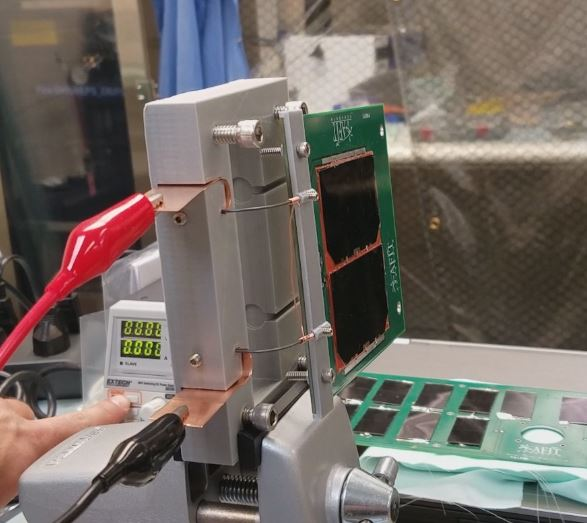
\includegraphics[width=0.305\linewidth]{Ch4/Figures/1U_Demo_1.jpg}
    \caption{Successful 1U demonstration of the Nitinol hinge prototype actuation}
	\label{f:1U_Demo}
\end{figure}
\FloatBarrier
%-----------------------------------------------------------------------



%	\chapter{Conclusions}
\label{chap:5}

%-----------------------------------------------------------------------
%Chapter 5 Conclusions and Recommendations
%-----------------------------------------------------------------------

% Nomenclature for Chapter 5
\nomenclature{$\beta$}{elevator deflection angle}

% Acronyms for Chapter 5
\newacronym{leo}{LEO}{Low-Earth Orbit}
\newacronym{gevs}{GEVS}{General Environmental Verification Specification}

%http://dissertationedd.usc.edu/the-purpose-of-chapter-5.html

%-----------------------------------------------------------------------
\section{Chapter Overview}
%-----------------------------------------------------------------------
% [WHY DOES IT MATTER]
% Write the introduction to include the problem, purpose, research questions and brief description of the methodology.

The United States Air Force's interest in disaggregated space architectures continues to grow. CubeSats are a very good vehicle for technology maturation and are becoming more attractive for real-world operations and tactical warfighting support. The power demand on CubeSats will undoubtedly continue to increase and this research is trying to address one small aspect of this issue.

CubeSat popularity in the aerospace industry continues to increase and so the expected number of small satellites will continue to grow. Therefore, satellite deployment mechanisms that prohibit the installations of more panels due to complexity and bulk requires the development of a more elegant method of deployment. Increase in popularity and the miniaturization of electronic components has driven power demands to the point that CubeSats will require additional solar panel folds to operate all of its electronics. The problem is, traditional CubeSat hinges are bulky and do not permit additional folds without encroaching into payload volume due to the increased thickness of their stowed configuration. For launch, CubeSats have to fit in a standardized CubeSat launcher or \gls{ppod}, making space constrained volume savings highly desired. Based on this research, a more sophisticated hinge utilizing Nitinol \gls{sma} could be used.  

The purpose of this thesis was to explore a solution to these problems with a Nitinol \gls{sma} hinge. This hinge design was able to demonstrate concept feasibility, and functionality, but not reduced complexity, or bulk.
% answer several research questions and research objectives which were: `Is the concept feasible?' `Does it reduce complexity, mass, and bulk?' and `Is it functional?' 
The research objectives were: Develop a Nitinol hinge design, manufacture a representative prototype, characterize its force properties, and identify areas of improvement.

The methodology of this work was first to learn how \gls{sma}s behave and determine the best way to work with them in order to be integrate them with a solar panel. For this, brainstorming sessions were held, and extensive preliminary testing was done to come up with an acceptable design. Then, it became a matter on how to best work with Nitinol and the  tools and material at hand. Several designs were built, and the lessons learned from that experience was used in building the final and simplest prototype. Finally, this prototype was used to conduct preliminary testing for movement and reaction times, and then on the actual force measurement experiments and relevant environment demonstrations, which lead to the reporting of the results and findings from the investigations.  

% \begin{description}
%  \item[$\bullet$]  \ Learn how the material works in theory
%  \item[$\bullet$]  \ Brainstorm designs 
%  \item[$\bullet$]  \ Figure out the best way to work with it
%  \item[$\bullet$]  \ Attempt to build designs by trial and error; Learn how to work with material
%  \item[$\bullet$]  \ Use lessons learned to build simplest prototype
%  \item[$\bullet$]  \ Do preliminary testing for movement, reaction times
%  \item[$\bullet$]  \ Run force measurement experiment
%  \item[$\bullet$]  \ Run demonstrations
%  \item[$\bullet$]  \ Report Findings and Results
% \end{description}

% From Chapter 1: Methodology Section
% To achieve the first objective of this research the author worked closely with \gls{afit} technicians to brainstorm Nitinol hinge designs and various heating techniques. To achieve the second objective, a series of trial and error experiments along with \gls{cad} will be used to spot areas of improvement to be incorporated into the existing design. For the third objective, a manufacturing schedule will be laid out and materials required not currently in-house will be ordered with the intent to build two prototypes. 
                                                                 

%-----------------------------------------------------------------------
\section{Discussion of Findings and Results}
%-----------------------------------------------------------------------
% Summary of Findings – In this discussion assert that you have answered your research questions.
% Summary of chapter 3 and 4 basically

This research demonstrated that the concept is feasible, and functional. However, at this early stage of technology development, the question of reduction of complexity, and bulk is still too early to answer. As it can be seen on the prototype, the radius of curvature of a 2 mm in diameter Nitinol rod is far too wide, at 12.1 mm, when compared to traditional hinge mechanisms that can fold 180\textdegree\ with a much smaller radius of curvature of 4.4 mm (as shown in Figure \ref{f:3U_Solar_Panel}). It was determined that the actuation volume for a Nitinol hinge with such a radius of curvature is about $7.864 \times 10^{-5}$ m$^3$, whereas a thin profile traditional spring hinge takes up only $5.675 \times 10^{-6}$ m$^3$. This is an order of magnitude less volume. %So the reduction in bulk is not quite there yet. As far as reduction in complexity, it is still undetermined. For integration, since soldering techniques failed, another mechanical way of integration had to be devised. 
Therefore, in order to be comparable, a further reduction in bulk is required. 
%This lead to the design and 3D printing of new solar panel holders to mount the solar panels to the test stand, so there were additional components incorporated onto the design which increased complexity and mass in a sense, but the concept still remains fairly simple.     
This reduction has to occur while also utilizing screws, crimps, and harnesses as use of these materials is the best method for integrating a Nitinol hinge.  
%-----------------------------------------------------------------------
\section{Research Impact}
%-----------------------------------------------------------------------
% US Air Force, formation flying, swarms of satellites, great numbers. 
% Increased of capability because more power is available with larger Solar Panels.

The implications of this research are directly related to the future of the U.S. Air Force space operations. The ability to pack larger solar panels in the small CubeSat form factor is critical to continually improve their capabilities and performance. For disaggregated platforms to work, power-hungry payloads will start working their way to ever smaller form factors to include the CubeSat standard and the ability to provide those payloads with sufficient power for their operations is critical. Additionally, with the larger number of satellites that such architecture requires, ways of minimizing debris generation is important to keep the space environment as particle free as possible which can degrade equipment and shorten the lifespan of orbiting space systems. Further development of this technology can culminate in a more elegant solution to CubeSat solar panel deployment.     

%-----------------------------------------------------------------------
\section{Future Research Recommendations}
%-----------------------------------------------------------------------

There is certainly extensive of work ahead to perfect the use of \gls{sma}s for this application. One such series of testing that would make the proof of concept even more convincing is to test the hinge in a thermal vacuum chamber to simulate the thermal conditions of orbit and characterize its performance. A test could be devised to measure the force produced by the hinge in line of sight of the Sun and in the shade. This would inform the researchers if the Nitinol activation temperature needs to be changed for improved operations, how Nitninol operates in a vacuum, how the current-force relation reacts to such temperature swings, and if there is any material degradation such as embrittlement, or something similar. 

Further design work, to more seamlessly integrate solar panels with Nitinol and Nitinol with the CubeSat bus should be explored further in order to work the issues of bulk and complexity which were left unresolved in this first iteration. Also, vibration testing of a deployed panel and hinge should be considered. Moreover, further packing and integration engineering is necessary to refine an efficient method to stow large, foldable solar arrays that uses Nitinol hinges. This vibration testing would also ensure that the \gls{nasa} \gls{gevs} standards are met adding confidence to its viability after going through the traumatic experience of launch. This would raise overall confidence of this proof of concept.  

To finalize, the possibility of utilizing two-way \gls{sma} on the hinge is enticing. Two-way \gls{sma} can move back and forth from two preset positions. This could be of interest for future solar panel actuation possibly eliminating the use of solar array drive assemblies, or utilizing temperature phasing for a passive control system. 

% If time allows, characterize dynamic behavior when subjected to the launch and space environment, and finally verify its viability and proper functioning after thermo-vacuum and vibration testing.  
% - Does it survive the launch and space environment?
% - Verify survivability of launch and space environment 
%  --Characterize its dynamic behavior when subjected to the launch and space environment
% - Verify its viability and proper functioning after thermo-vacuum and vibration testing

% For the fourth and fifth objectives one of the two prototypes will be used for extensive environmental testing in an attempt to increase confidence in the community of its use. 

% , thermo-vacuum chamber, and vibration testing table.

% [The difference between the two 2.2A and 12V tests, why is that. Is there material degradation?]

%-----------------------------------------------------------------------
\section{Conclusions}
%-----------------------------------------------------------------------
Much was learned by embarking on this research, especially of the legacy that \gls{sma}s have starting in the 1960's and of their peculiar material properties. Their use has expanded to many industries and in the 1990's its application has really taken off to a much wider variety of use. The aerospace industry is at the forefront of innovation and by investigating additional uses of \gls{sma}s in CubeSats that tradition is continued. The U.S. Air Force has much to gain from this research as its interest in small satellites increases for disaggregated space architectures, and rapid technology development. This research has demonstrated that a Nitinol hinge for CubeSat solar panels is feasible and functional, but its design has to be refined in order to be practical.    

% %-----------------------------------------------------------------------
% \section{Equations}
% %-----------------------------------------------------------------------
    
% \begin{equation}
% \label{e:visc}
% \tau_{xy}=\mu\frac{d\theta}{dt}=\mu\frac{du}{dy}
% \end{equation}
% \nomenclature{$\tau_{xy}$}{Shear Stress}
% \nomenclature{$\mu$}{Dynamic Viscosity}

% It may sometimes be best to use subequations as opposed to a single equations, depending on context. Equations and sub equations can easily be referenced. The nomenclature package allows calling of variables where they are used. There are ways to define classes of variables to be listed together in the nomenclature, but time is probably better spent elsewhere. An alternative method is to define symbols as acronyms so that the same rules are used for extended definitions. That way is stupid and inefficient. If you want to math it up in the text, simply use \$ on either side of the commands like $q=\frac{1}{2}\rho V^2$.

% \begin{subequations}
% 	\begin{equation}
% 	\label{e:Rey_dyn}
% 	Re=\frac{\rho VL}{\mu}
% 	\end{equation}
% 	\begin{equation}
% 	\label{e:Rey_kin}
% 	Re=\frac{VL}{\nu}
% 	\end{equation}
% \end{subequations}
% \nomenclature{$Re$}{Reynolds Number}
% \nomenclature{$\rho$}{Density}
% \nomenclature{$V$}{Fluid Velocity}
% \nomenclature{$L$}{Characteristic Length}
% \nomenclature{$\nu$}{Kinematic Viscosity}

% For those trying to do more advanced math commands, \verb|\begin{aligned}| starts an environment that aligns equations to \& placement. Something like this can be used to align a family of equations to the = sign as shown below.

% \begin{equation}
% \begin{aligned}
% D=& 140\quad in=3.556\quad m\\
% \rho=&1.18\quad\frac{kg}{m^3}\\
% \mu=& 18\times10^{-6}\quad \frac{kg}{m\cdot s}\\
% t=&120\quad days=2880\quad hrs 
% \end{aligned}
% \tag{\ref{e:Rey_dyn} revisited}
% \label{e:wrong}
% \end{equation}

% The aligned environment can be contained in braces as shown below, but brackets, parenthesis, etc. will work as well. Notice how in that last equation I manually defined the tag to \ref{e:wrong}, and referenced it to one of the previous equations.

% \begin{equation}
% N=\left\lbrace\begin{aligned}
% N_{10}\\  % Notice that subscripts of multiple characters need to be in {}'s
% N_{20}\\
% N_{40}
% \end{aligned}\right\rbrace=\left\lbrace\begin{aligned}
% 10\\
% 20\\
% 40\end{aligned}\right\rbrace RPM\quad=\quad\left\lbrace\begin{aligned}
% 0.167\\
% 0.333\\
% 0.667
% \end{aligned}\right\rbrace\frac{rev}{s}
% \end{equation}
% \nomenclature{$N_i$}{Rotational Rate, Indexed}

% Discussion: Characterize its force properties. Experiment


\appendix
%	%\newpage
\chapter{Force Measurement Test Calibration Data} 
\label{App:AppendixA}

% Please add the following required packages to your document preamble:
% \usepackage{booktabs}

\begin{table}[htbp]
\centering
\caption{Force Measurement Calibration Data}
\label{CalData}
\begin{tabular}{@{}llll@{}}
\toprule
\textbf{Mass (g)} & \textbf{Voltage (V)} & \textbf{Mass (g)} & \textbf{Voltage (V)} \\ \midrule
50                & 2.00E-08             & 550               & 3.25E-07             \\
70                & 3.00E-08             & 570               & 3.30E-07             \\
80                & 4.00E-08             & 1000              & 5.95E-07             \\
500               & 2.85E-07             & 1050              & 6.20E-07             \\
510               & 2.95E-07             & 1080              & 6.40E-07             \\
520               & 3.00E-07             & 1500              & 8.95E-07             \\
530               & 3.05E-07             & 1550              & 9.40E-07             \\ \bottomrule
\end{tabular}
\end{table}



%	\include{AppendixB/thesis-AppB}
%	\include{AppendixC/thesis-AppC} 
%	\include{AppendixD/thesis-AppD} 
%	\include{AppendixE/thesis-AppE} 

\bibliographystyle{aiaa}
\bibliography{Mendeley}

% SF298, but in Front Matter folder
\backmatter
%        \singlespace                                       
%        \setlength\bibsep{\baselineskip}
%        \bibliographystyle{apacite}
%        \renewcommand\bibname{Bibliography}
%        \bibliography{Ocampo_bibtex_thesis.bib} 

%	\date{March 2019}
\ReportDate{??--03--2019} \ReportType{Master's Thesis}
\DatesCovered{Sept 2017 --- Mar 2019}

\Title{\centering Fragmentation Properties of Explosively Driven\\
        Additively Manufactured Materials}

%\Title{\centering \MakeUppercase{Evaluation of Interplanetary
%Magnetic Field Tracing Models Using Impulsive SEP's}}

%\ContractNumber{DACA99--99--C--9999}

%\GrantNumber{}
%\ProgramElementNumber{}
%\ProjectNumber{09ENP???}
%\TaskNumber{}
%\WorkUnitNumber{}

\Author{LeSieur, Alexander R., Captain, USAF}


\PerformingOrg{Air Force Institute of Technology\\[-1pt]
    Graduate School of Engineering and Management (AFIT/EN)\\[-1pt]
    2950 Hobson Way\\[-1pt]
    WPAFB OH 45433-7765}

\POReportNumber{AFIT-ENY-MS-19-M-XXX}

\SponsoringAgency{Intentionally Left Blank\\[-1pt]}
% Att: Major Ryan P. O'Hara\\[-1pt]
% 2950 Hobson Way\\[-1pt]
% WPAFB OH 45433\\[-1pt]
% Email: ryan.ohara@afit.edu }

\Acronyms{}
%\SMReportNumber{}
\DistributionStatement{DISTRIBUTION STATEMENT A:\\[-1pt]
\MakeUppercase{Approved for Public Release; distribution unlimited.}}

\Abstract{Fragmentation properties are a crucial component of military weaponeering, where the fundamental goal is to create the optimal weapons package for mission accomplishment, while minimizing collateral damage. Additive manufacturing presents an avenue towards tailoring a warhead's design to a specific target set, allowing weapons experts to develop efficient attack solutions, further reducing unintended consequences, while improving aircraft survivability. Understanding the fragmentation properties of additively manufactured materials under explosive loading is needed before they are utilized in weaponry applications. This research will examine the fracture behavior of metal casings produced by additive manufacturing and the resulting fragment velocity and mass distributions through experimental analysis.
 \textemdash Alexander LeSieur, Capt, USAF\\ [-10pt]} 

\SubjectTerms{Additive Manufacturing, }

\NumberPages{XX}
%\ReportClassification{}
%\PageClassification{}
%\AbstractClassification{}
\AbstractLimitation{UU}

\ResponsiblePerson{Major , AFIT/ENY}

\RPTelephone{(937) 255-3636, x4XXX; @afit.edu}

\MakeRptDocPage

	
	
\end{document}
